
%(BEGIN_QUESTION)
% Copyright 2015, Tony R. Kuphaldt, released under the Creative Commons Attribution License (v 1.0)
% This means you may do almost anything with this work of mine, so long as you give me proper credit

This P\&ID shows the control system for a {\it fractionator} (otherwise known as a {\it distillation column} whereby a multi-component liquid is separated into its constituent components by boiling and condensing.  The incoming ``feed'' is pre-heated by a gas-fired ``charge heater'' unit (not shown in this diagram), then heated more by passing through a bank of heat exchangers (E-5 through E-7) cooling off distilled product while heating incoming feed, and then introduced into the middle of the fractionator vessel (C-5) where the lighter fractions rise up and the heavier fractions fall down to be collected at different heights along the vessel.  ``Bottoms'' liquid at the bottom of the fractionator is re-boiled by a steam-heated exchanger (E-9) while ``Overhead'' vapors are condensed by a water-cooled exchanger (E-8) and collected in an accumulator vessel (V-13), some of which is re-introduced into the fractionator as ``reflux'' flow:

$$\includegraphics[width=15.5cm]{i0001rx01.eps}$$

Feed flow transmitter FT-40 plays an important role in this control system, monitoring the rate at which fresh feed enters the fractionator tower.  This flow signal is used in multiple feedforward control schemes in this system.  Identify those feedforward systems and explain what they do.

\vskip 10pt

Also identify where {\it dynamic compensation} is employed in this system, and explain the purpose for doing so.

\vskip 10pt

Finally, explain how you would ``tune'' the feedforward systems for the correct amount of action, and also ``tune'' the dynamic compensation for the correct amount of time.

\underbar{file i02885}
%(END_QUESTION)





%(BEGIN_ANSWER)

FT-40's signal is fed forward into two control loops: FFC-41 (Flow Ratio Controller \#41) which controls the flow of heating steam to the reboiler, and FC-34 (Flow Controller \#34) which controls the flow of distillate (overhead) product exiting the system.  The concept here is that additional feed flow into the fractionator demands additional heat applied to the reboiler as well as additional heat removed from the system in the form of overhead product drawn away from the fractionator.

\vskip 10pt

We see dynamic compensation applied to this feedforward signal in the form of lead/lag functions FY-40a and FY-40b.  FY-40a applies lead/lag to the reboiler steam flow controller while FY-40b applies lead/lag to the distillate product flow controller.  The concept here is that changes in feed flow, while demanding commensurate changes in reboiler steam flow and distillate product flow, will not impose a loading effect with the same lag time as an immediately fed-forward command to change steam and distillate flow rates.  Therefore, these lead/lag functions must add some lag time to the feedforward signal (essentially delaying its effect) so that it does not over-compensate immediately following a change in feed flow rate.

\vskip 10pt

``Tuning'' any feedforward system requires that you disable any feedback control (so that you will be monitoring pure feedforward action) and then introduce intentional load changes to watch the feedforward compensation.  This means de-tuning FFC-41 (i.e. setting its PID parameters for minimum effect) and watching changes in reboiler temperature as the feed flow (load) is changed, as well as de-tuning FC-34 and watching for changes in overhead accumulator (V-13) liquid level.  Under-compensation should be corrected by increasing feedforward gain, while over-compensation should be corrected by decreasing that gain.  Lag time and the lead/lag ratio should be adjusted such that there is minimal over/under compensation transients following a load change.

%(END_ANSWER)





%(BEGIN_NOTES)

Control strategy based on that shown on page 1179 of B\'ela Lipt\'ak's {\it Instrument Engineer's Handbook, Process Control}, Third Edition.  Embellishments added just to make the diagram more evil!

\vskip 20pt \vbox{\hrule \hbox{\strut \vrule{} {\bf Virtual Troubleshooting} \vrule} \hrule}

This question is a good candidate for a ``Virtual Troubleshooting'' exercise.  Presenting the diagram to students, you first imagine in your own mind a particular fault in the system.  Then, you present one or more symptoms of that fault (something noticeable by an operator or other user of the system).  Students then propose various diagnostic tests to perform on this system to identify the nature and location of the fault, as though they were technicians trying to troubleshoot the problem.  Your job is to tell them what the result(s) would be for each of the proposed diagnostic tests, documenting those results where all the students can see.

During and after the exercise, it is good to ask students follow-up questions such as:

\begin{itemize}
\item{} What does the result of the last diagnostic test tell you about the fault?
\item{} Suppose the results of the last diagnostic test were different.  What then would that result tell you about the fault?
\item{} Is the last diagnostic test the best one we could do?
\item{} What would be the ideal order of tests, to diagnose the problem in as few steps as possible?
\end{itemize}

%INDEX% Control, strategies: feedforward with dynamic compensation (lead/lag)
%INDEX% Process: distillation, generic (realistic P&ID shown)

%(END_NOTES)

